\documentclass[10pt,a4paper]{article}
\usepackage[latin1]{inputenc}
\usepackage{amsmath}
\usepackage{amsfonts}
\usepackage{amssymb}
\usepackage[]{theorem}
\usepackage[nottoc]{tocbibind}
\usepackage[hidelinks]{hyperref}
\usepackage{appendix}
\usepackage{listings}
%\usepackage{minitoc}
\usepackage{graphicx}
\usepackage{float}
\usepackage{makecell}
\usepackage{authblk}
\usepackage[bottom]{footmisc}

\setlength{\topmargin}{-.5in}
\setlength{\textheight}{9in}
\setlength{\oddsidemargin}{.125in}
\setlength{\textwidth}{6.25in}

\newcommand {\subsubsubsection} [1] {\vskip 0.5em {\bf \em #1}}

%\newcommand {\comm} [1] {}
\newcommand {\comm} [1]
{
\par
\setlength{\leftskip}{-0.8in}
\begin{tabular} {p{0.1cm} | p{\textwidth}}
  {\bf ?} & {#1}
\end{tabular}
\par
\setlength{\leftskip}{0in}
}


\newcommand {\cond} {, & \textrm{if }}
\newcommand {\otherwise} {, & \textrm{else}}

\newcommand {\Forall} {\forall \ }
\newcommand {\eqdef} {\triangleq}
\newcommand {\equivalent} {\Leftrightarrow}
\renewcommand {\implies} {\Rightarrow}
\renewcommand {\impliedby} {\Leftarrow}
\renewcommand {\And}  {\ \& \ }
\newcommand {\Or}  {\ \vee \ }
\newcommand {\QED} {$\square$ \ \par }
\newcommand {\proofword}  {{\par \sf Proof:\ }}
\newcommand {\proof} [1] {\proofword #1 \QED \par}
\newcommand {\definition} [2] {\bigskip {\bf Definition} {\rm \sc #1} \par #2 \QED \bigskip}
\newcommand {\example} [2] {\bigskip {\bf Example.} {#1} \par #2 \QED}
\newcommand {\theorem} [2] {\bigskip {\bf Theorem} {\rm \sc #1} \par #2 \QED \bigskip}
\newcommand {\ve} {\mathbf}
\newcommand {\vecc} {\boldsymbol}
\newcommand {\Questions} {\vspace{5mm} {\bf Unresolved Questions:}}
\newcommand {\assert} {\square \ }

\renewcommand {\P} {\mathrm P}
\newcommand {\E} {\mathrm E \ }
\newcommand {\var} {\mathrm {var} \ }
\newcommand {\cov} {\mathrm {cov} }
\newcommand {\cor} {\mathrm {cor} }
\newcommand {\N} {\mathbb N}
\newcommand {\Z} {\mathrm Z}
\newcommand {\R} {\mathbb R}
\newcommand {\C} {\mathbb C}
\newcommand {\I} {\mathbb I}
\newcommand {\supp} {\mathrm {Supp}}
\newcommand {\mat} {\mathrm}
\newcommand {\trc} {\mathrm {tr} \ }
\newcommand {\VC} {\mathrm {VC} }
\newcommand {\const} {\mathrm {const} }
\newcommand {\sgn} {\mathrm {sgn} }
\newcommand {\dom} {\mathrm {dom} }
\newcommand {\range} {\mathrm {range} }
\newcommand {\Arg} {\mathrm {Arg} \ }

\newcommand {\LCA} {\mathrm {LCA} }  % least common ancestor (in a tree)

\newcommand {\nul} {\mathrm {null}}
\newcommand {\Dt} {\Delta t}
\newcommand {\PC} {\mathrm {PC} }
\newcommand {\MDS} {\mathrm {MDS} }
\newcommand {\CC} {\mathrm {CC} }

\newcommand {\re} {\mathrm {re}}
\newcommand {\cl} {\mathrm {cl}}
\newcommand {\intr} {\mathrm {int}}

\newcommand {\<} {\langle}
\renewcommand {\>} {\rangle}

\newcommand {\dotve} [1] {\dot {\ve #1}}

\newcommand {\la} [1] {\lambda (#1) \ }

\newcommand {\lhs} {\mathrm {lhs}}
\newcommand {\rhs} {\mathrm {rhs}}

\providecommand{\keywords}[1]
{
  \small
  \textbf{\textit{Keywords---}} #1
}

\makeatletter
\DeclareRobustCommand{\cev}[1]{%
  {\mathpalette\do@cev{#1}}%
}
\newcommand{\do@cev}[2]{%
  \vbox{\offinterlineskip
    \sbox\z@{$\m@th#1 x$}%
    \ialign{##\cr
      \hidewidth\reflectbox{$\m@th#1\vec{}\mkern4mu$}\hidewidth\cr
      \noalign{\kern-\ht\z@}
      $\m@th#1#2$\cr
    }%
  }%
}
\makeatother



\providecommand{\keywords}[1]
{
  \small	
  \textbf{\textit{Keywords---}} #1
}


\title{Phylogenetic Tree of SARS-CoV-2 Complete Sequences}
\author[1]{Slava Brover\footnote{E-mail: brovervv@ncbi.nlm.nih.gov}}
\affil[1]{\small National Center of Biotechnology Information, National Institutes of Health, 9600 Rockville Pike, Bethesda, MD, 20892, USA}


\begin{document}
\maketitle

\begin{abstract}
Phylogenetic tree of SARS-CoV-2 sequences deposited at NCBI is built by a distance optimization.
Mutations relative to the reference sequence are used for the computation of dissimilarities between pairs of sequences.
\end{abstract}

\keywords {SARS-CoV-2, Covid, Phylogeny, Distance Tree, Mutation.}

%\dominitoc
%\tableofcontents



\section {Materials}

The phylogenetic tree of complete SARS-CoV-2 sequences is a distance tree built incrementally using the tool~\cite{inc_ls_dist_tree}.

The SARS-CoV-2 sequences deposited at NCBI~\cite{Virus}
are downloaded daily
from \url {https://www.ncbi.nlm.nih.gov/labs/virus/vssi/#/virus?SeqType\_s=Nucleotide&VirusLineage\_ss=Severe\%20acute\%20respiratory\%20syndrome\%20coronavirus\%202,\%20taxid:2697049},
and if the new sequences make up at least~1~\% of the old sequences
they are added to the phylogenetic tree.

Each sequence is identified by an NCBI accession 
and has the following metadata fields:
\begin{itemize}
  \item Host;
  \item Isolation Source;
  \item Country extracted from GeoLocation;
  \item Collection Date;
  \item Publication Date.
\end{itemize}


\section{Methods}

The sequences are aligned with the reference SARS-CoV-2 sequence NC\_045512.2 without polyA,
the unaligned parts, i.e., linker and polyA, are trimmed,
and {\em raw} mutations are identified.

For example, the set of raw mutations of the sequence LC528232.1 is
$$\{\mathrm {t3g, gg7at, t13DEL, c15t, t18DEL, g11083t}\}, $$
and the set of raw mutations of the sequence MT114418.1 is
$$\{\mathrm {c8092t, g11083t}\}.$$
The raw mutation ``gg7at'' in LC528232.1 means that the nucleotides ``gg'' in the reference sequence starting at position~7 are replaced by the nucleotides ``at'' in LC528232.1.
In other words, the segment 7-8 of the reference sequence is replaced by ``at''.
A raw mutation ``xnDEL'' is a {\em deletion},
and a raw mutation ``INSny'' is an {\em insertion}.

A raw mutation is {\em ambiguous} if the nucleotides of the reference sequence are replaced by at least one ambiguous nucleotide.
A deletion ``xxx1DEL'' means a truncation of the reference sequence at~5' end,
and it is replaced by the raw mutation ``xxx1nnn''.

% Unaligned target ends are not observed, probably because all targets have already been aligned to the reference before depositing to GenBank.

It is assumed that polyAs are trimmed correctly and, therefore, the sequences have complete~3' ends.

For each sequence raw mutations are replaced by {\em clean} mutations using the following rules:
\begin{itemize}
  \item For non-ambiguous raw mutations the clean mutations are the same. 
        These clean mutations are {\em present} in the sequence;
  \item Each ambiguous raw mutation is replaced by all non-ambiguous raw mutations of other sequences within the same segment.
        These clean mutations are {\em optional} in the sequence.
        In other words, these clean mutations may or may not be present in the sequence
        because they are located in low-quality regions of the sequence.
  For example, the mutation ``atta1DEL'', 
  which means that the segment 1-4 of the reference sequence is missing,
  is replaced by the following clean optional mutations which are present in other sequences:
$$\{\mathrm {tt2aa, tta2gct, t2g, t3a, t3g, INS3g, t3c, ta3gg, a4c, a4t, a4g}\}. $$
\end{itemize}

Clean mutations contain only non-ambiguous nucleotides.

Let~$M$ be the set of all clean mutations in the available set~$S$ of sequences.
Then the assignment of clean mutations to sequences defines a function 
$$\chi : S, M \mapsto B_3,$$
where $B_3 = \{present, optional, absent\}$.
This means that each sequence has a 3-valued Boolean vector of clean mutations in~$M$.
And the Hamming dissimilarity between sequences~$x$ and~$y$ is defined as
$$ H_\alpha(x,y) = \sum_{m \in M} \delta_\alpha(\chi(x,m),\chi(y,m)), $$
where $0 \le \alpha \le 1$
and the difference function $\delta_\alpha : B_3, B_3 \mapsto [0,1]$ is defined in Table~\ref{tab:d}.

\begin{table}[H]
  \centering
  \begin{tabular}{|l|c|c|c|}
    \hline
                   & $present$ & $optional$ & $absent$ \\
    \hline
    $present$      &  0         & $\alpha$  & 1 \\
    $optional$     & $\alpha$   & 0         & 0 \\
    $absent$       & 1          & 0         & 0 \\
    \hline
  \end{tabular}
  \caption{Difference function $\delta_\alpha : B_3, B_3 \mapsto [0,1]$.}
  \label{tab:d}
\end{table}

For example, $H_\alpha(\mathrm{LC528232.1},\mathrm{MT114418.1}) = 6$ for any~$\alpha$.

The phylogenetic tree is optimized
with the optimization criterion which is the fitness of the tree distances to the dissimilarities between sequences:
$$ \sum_{x,y} (d_{xy} - l_{xy})^2 \ \frac 1 {v_{xy}}, $$
where~$(x,y)$ are pairs of sequences,
$d_{xy}$ is the dissimilarity between~$x$ and~$y$,
$l_{xy}$ is the tree distance between~$x$ and~$y$,
and
$v_{xy}$ is the dissimilarity variance of the pair $(x,y)$.
This criterion is minimized.

The expressions for~$d$ and~$v$ are chosen so that the miscongruence with reference classifications should be minimized, see~\cite{maxCongr}. 
The metadata fields were used as reference classifications.
The results of the parameter optimization for the initial 2,849 sequences are in Table~\ref{tab:param}.

% Use Jukes-Cantor model ??

\begin{table}[H]
  \centering
  \begin{tabular}{|c|c|c|}
    \hline
    Dissimilarity~$d$ & Dissimilarity variance~$v$ & \makecell {Miscongruence with \\ reference classifications} \\
    \hline
    & & \\[-1em]
    $H_{0.2}$      & $\max (l^{2.5}, 1)$     & 3078  \\
    $H_{0.2}$      & $\max (l^{2}, 1)$       & 3098  \\
    $H_{0.2}$      & $\max(l^{3}, 1)$        & 3088  \\
    $H_{0.2}$      & $\max(l^{2.5}, 0)$      & 3375  \\
    $H_{0.2}$      & $\max(l^{2.5}, 2)$      & 3103  \\
    $H_{0.0}$      & $\max (l^{2.5}, 1)$     & 3116  \\
    $H_{0.1}$      & $\max (l^{2.5}, 1)$     & 3094  \\
    $H_{0.3}$      & $\max (l^{2.5}, 1)$     & 3090  \\
    $H_{0.4}$      & $\max (l^{2.5}, 1)$     & 3106  \\
    \hline
  \end{tabular}
  \caption{Optimization of the distance tree parameters: the top row contains the best parameters.
    Not all tried combinations are in this table.}
  \label{tab:param}
\end{table}

Only those trimmed sequences are used in the tree building which satisfy the following quality criteria:
\begin{itemize}
  \item Collection Date must exist;
  \item sequence length must be between 29600 and 31000 bp;
  \item the fraction of ambiguous nucleotides in sequences must be below 1~\%;
\end{itemize}

After the tree has been optimized,
it is rooted so that Collection Dates must be most consistent with the tree.
This is achieved by solving a maximum parsimony problem 
with Collection Dates rounded to 1st, 10th and 20th days 
and converted to 3-valued Boolean attributes.


\section{Results}

The latest incrementation of the tree is available at
\url {https://www.ncbi.nlm.nih.gov/labs/virus/vssi/#/precomptree}
in Newick format
where the metadata fields are added.
The tree built on January 23, 2021 has 38,025 SARS-CoV-2 complete sequences.

For the obtained distance tree
the clean mutations are used as 3-value Boolean attributes for the maximum parsimony problem on this tree.
The solution to this problem assigns subsets of clean mutations of~$M$ to the interior nodes of the tree.
A mutation is {\em gained} if it is assigned to a node, but it is not assigned to its parent node,
and a mutation is {\em lost} if it is not assigned to a node, but it is assigned to its parent node,
At each tree arc the gained or lost clean mutations are displayed with the prefix~``+'' or~``-'',
see Fig.~\ref{fig:Tree}.

\begin{figure}[h]
  \centering
  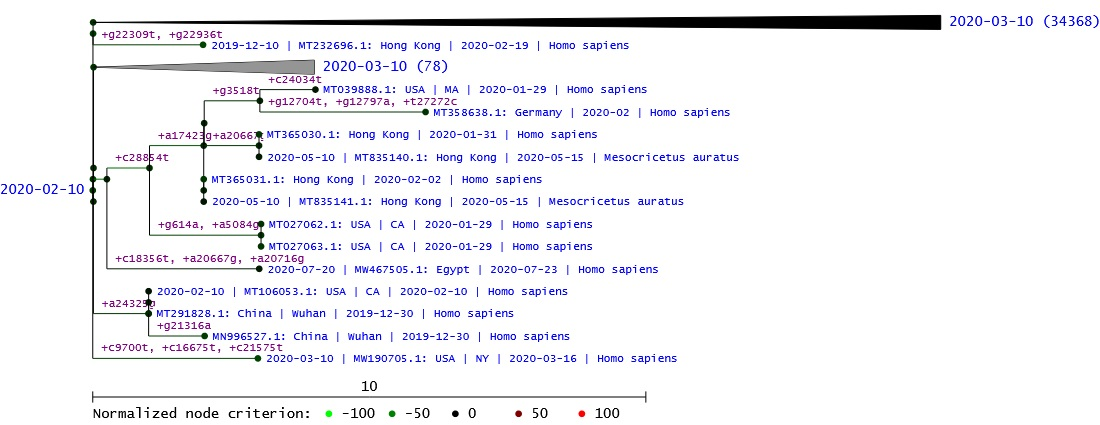
\includegraphics[scale=0.6]{Covid.jpg}
  \caption{SARS-CoV-2 tree with gained or lost clean mutations.}
  \label{fig:Tree}
\end{figure}


Distribution of gained mononucleotide mutations of the tree of January 23, 2021 is in Table~\ref{tab:SNP}.
This table shows a tendency for ``c'' and ``g'' to mutate into ``t'' 
so that GC\% decreases with the rate of~0.04\% per year, 
see Fig.~\ref{fig:CG}.

\begin{table}[H]
  \centering
  \begin{tabular}{|c|r|r|r|r|}
    \hline
From\textbackslash To &   a &   c &    g & t \\
\hline
a        &   - & 653 & 3700 & 825 \\
c        & 892 &   - &  161 & 19692 \\
g        & 3189& 588 &    - & 7906 \\
t        & 703 &3855 &  527 & - \\
    \hline
  \end{tabular}
  \caption{Number of gained mononucleotide mutations.}
  \label{tab:SNP}
\end{table}


\begin{figure}[h]
  \centering
  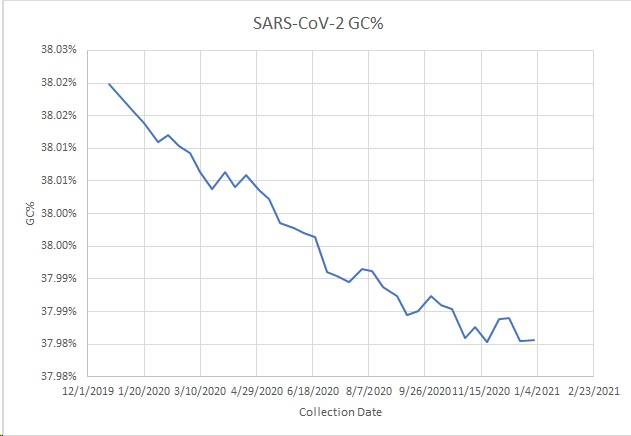
\includegraphics[scale=0.8]{CG.jpg}
  \caption{Dependence of GC\% on Collection Date.}
  \label{fig:CG}
\end{figure}
 



\section*{Funding}
This research was supported by the National Center for Biotechnology Information of the National Library of Medicine (NLM), National Institutes of Health.


\section*{Availability of data and materials}
The latest incrementation of the tree is available at
\url {https://www.ncbi.nlm.nih.gov/labs/virus/vssi/#/precomptree}.


\section*{Authors contributions}
Not applicable.


\section*{Competing interest}
Authors declare that they have no competing interests.


\section*{Consent for publication}
Not applicable.


\section*{Ethics approval and consent to participate}
Not applicable.




\clearpage
\begin{thebibliography}{9}

\bibitem{Virus}
Virus Variation Resource - improved response to emergent viral outbreaks.
Hatcher EL, Zhdanov SA, Bao Y, Blinkova O, Nawrocki EP, Ostapchuck Y, Sch�ffer AA, Brister JR.
Nucleic Acids Res. 2017 Jan 4;45(D1):D482-D490. doi: 10.1093/nar/gkw1065. Epub 2016 Nov 28. 

\bibitem{inc_ls_dist_tree}
Brover~S.,
Building Large Phylogenetic Trees in Log-Linear Time,
{\it in print.}


\bibitem{maxCongr}
Brover~S.,
Principle of a Congruence Maximization of a Phylogenetic Tree to Reference Classifications,
{\it in print}
 


\end{thebibliography}


\bibliographystyle{unsrt}



\end{document}


